\subsection*{Tuần 4}

\subsubsection*{4.1 Mô tả công việc}

Trong tuần 4 của kỳ thực tập, sinh viên được giao nhiệm vụ khảo sát phần cứng của máy lọc nước Truliva nhằm xây dựng phương án thu thập dữ liệu phục vụ hệ thống giám sát thiết bị từ xa. Các công việc được thực hiện bao gồm:

\begin{itemize}
    \item Khảo sát cấu trúc tổng thể của máy lọc nước Truliva, xác định chức năng của các thành phần phần cứng như bo mạch điều khiển, bo hiển thị, cảm biến, bơm, van điện từ và các module liên quan.
    
    \item Phân tích kiến trúc hệ thống điều khiển, nghiên cứu các giao tiếp giữa các bo mạch và xác định các vị trí có thể khai thác dữ liệu phục vụ cho hệ thống IoT.
    
    \item Đánh giá các phương án tích hợp IoT vào thiết bị, phân tích ưu điểm, nhược điểm của việc can thiệp trực tiếp vào bo mạch điều khiển và phương án sử dụng vi điều khiển độc lập.
    
    \item Phân tích những khó khăn trong quá trình tích hợp, bao gồm cấu trúc phần cứng phức tạp, hạn chế về tài liệu kỹ thuật của một số linh kiện và các rủi ro khi can thiệp vào hệ thống điều khiển hiện có.
    
    \item Thiết kế phương án sử dụng vi điều khiển ESP32 làm bộ thu thập dữ liệu, xác định các tín hiệu đầu vào, nguồn cấp, sơ đồ kết nối với cảm biến và các giao tiếp cần thiết để truyền dữ liệu.
    
    \item Nghiên cứu phương án truyền dữ liệu từ ESP32 lên nền tảng IoT thông qua giao thức MQTT, tìm hiểu cách kết nối với HiveMQ Broker, tổ chức topic, định dạng bản tin JSON và quy trình gửi dữ liệu đến hệ thống giám sát.
    
    \item Xây dựng kiến trúc tổng thể của luồng dữ liệu từ thiết bị, ESP32, HiveMQ Broker đến hệ thống Device Monitor, làm cơ sở cho việc phát triển và triển khai ở các tuần tiếp theo.
\end{itemize}


\subsubsection*{4.2 Nội dung thực hiện}

\subsubsubsection*{4.2.1 Bối cảnh}

Dự án SmartWater hướng đến xây dựng hệ thống giám sát và quản lý máy lọc nước Truliva thông qua nền tảng IoT, cho phép theo dõi trạng thái hoạt động của thiết bị từ xa, thu thập dữ liệu vận hành và hỗ trợ công tác bảo trì. Để đáp ứng yêu cầu này, hệ thống cần có khả năng thu thập dữ liệu từ phần cứng của máy lọc nước và truyền về máy chủ để xử lý.

Trước khi triển khai giải pháp IoT, cần khảo sát cấu trúc phần cứng của thiết bị nhằm xác định kiến trúc điều khiển, các thành phần điện tử, giao tiếp giữa các bo mạch và khả năng khai thác dữ liệu. Kết quả khảo sát sẽ là cơ sở để đánh giá tính khả thi của các phương án tích hợp và lựa chọn giải pháp phù hợp.

Vì vậy, trong tuần 4, sinh viên tập trung nghiên cứu phần cứng máy lọc nước Truliva, phân tích hệ thống điều khiển và đề xuất phương án thu thập dữ liệu phục vụ cho các giai đoạn phát triển tiếp theo.
\subsubsubsection*{4.2.2 Khảo sát phần cứng máy lọc nước}

\textbf{Mục tiêu khảo sát}

Trước khi triển khai hệ thống IoT, sinh viên tiến hành khảo sát phần cứng của máy lọc nước Truliva nhằm hiểu rõ cấu trúc thiết bị, nguyên lý hoạt động và xác định các vị trí có thể thu thập dữ liệu. Kết quả khảo sát là cơ sở để đánh giá khả năng tích hợp hệ thống IoT mà không làm ảnh hưởng đến hoạt động của máy.

\vspace{0.5em}

\textbf{Khảo sát cấu trúc tổng thể}

Qua quá trình khảo sát thực tế, máy lọc nước Truliva được xác định gồm nhiều module phần cứng phối hợp với nhau để thực hiện chức năng điều khiển, hiển thị và giám sát trạng thái hoạt động. Các thành phần chính bao gồm:

\begin{itemize}
    \item Bo mạch điều khiển trung tâm (Main Control Board).
    \item Bo hiển thị và giao tiếp người dùng.
    \item Hệ thống cảm biến.
    \item Bơm tăng áp, van điện từ và các cơ cấu chấp hành.
    \item Nguồn cấp và hệ thống dây tín hiệu.
\end{itemize}

Trong đó, hệ thống điều khiển sử dụng hai bo mạch chính gồm bo điều khiển UR S61298 và bo hiển thị UR S61296. Hai bo mạch này đảm nhiệm các chức năng điều khiển thiết bị, hiển thị trạng thái hoạt động và trao đổi dữ liệu thông qua các đường truyền tín hiệu nội bộ.

\vspace{0.5em}

\textbf{Khảo sát bo điều khiển UR S61298}

Bo mạch UR S61298 là bo điều khiển trung tâm của máy lọc nước, chịu trách nhiệm tiếp nhận tín hiệu từ các cảm biến, điều khiển các cơ cấu chấp hành như bơm và van điện từ, đồng thời xử lý logic vận hành của thiết bị. Trên bo mạch tích hợp vi điều khiển, các mạch nguồn, mạch điều khiển công suất và các đầu nối giao tiếp với những module khác trong hệ thống.

\vspace{0.5em}

\textbf{Khảo sát bo hiển thị UR S61296}

Bo mạch UR S61296 đảm nhận chức năng giao tiếp với người sử dụng thông qua hệ thống đèn LED báo trạng thái và các nút nhấn điều khiển như \textit{Reset} và \textit{Select}. Bo mạch được kết nối với bo điều khiển thông qua đầu nối 6 chân gồm nguồn cấp, mass và các đường truyền nhận dữ liệu, cho phép đồng bộ trạng thái hoạt động giữa hai bo mạch.

\vspace{0.5em}

\textbf{Khảo sát các cảm biến và tín hiệu}

Sinh viên tiến hành xác định các tín hiệu đầu vào của hệ thống như cảm biến chất lượng nước (TDS), cảm biến lưu lượng, trạng thái lõi lọc và các tín hiệu cảnh báo. Đồng thời, các đường truyền tín hiệu giữa cảm biến và bo điều khiển cũng được khảo sát nhằm đánh giá khả năng thu thập dữ liệu phục vụ hệ thống IoT.

\vspace{0.5em}

\textbf{Kết quả khảo sát}

Kết quả khảo sát cho thấy máy lọc nước Truliva có cấu trúc phần cứng được thiết kế theo dạng module, trong đó bo UR S61298 đóng vai trò điều khiển trung tâm và bo UR S61296 đảm nhiệm chức năng hiển thị. Hai bo mạch trao đổi dữ liệu thông qua giao tiếp nội bộ, tạo nền tảng để nghiên cứu khả năng thu thập dữ liệu và tích hợp hệ thống IoT trong các bước tiếp theo.
\subsubsubsection*{4.2.3 Phân tích hệ thống điều khiển}

Sau khi hoàn thành quá trình khảo sát phần cứng, sinh viên tiến hành phân tích kiến trúc điều khiển của máy lọc nước Truliva nhằm xác định nguyên lý hoạt động của hệ thống, mối liên kết giữa các bo mạch và các vị trí có thể khai thác dữ liệu phục vụ cho việc tích hợp IoT.

\vspace{0.5em}

\textbf{Kiến trúc điều khiển}

Qua quá trình khảo sát, hệ thống điều khiển được xác định gồm hai bo mạch chính:

\begin{itemize}
    \item \textbf{Bo điều khiển UR S61298}: đóng vai trò là bộ điều khiển trung tâm, tiếp nhận tín hiệu từ các cảm biến, xử lý logic điều khiển và điều khiển các cơ cấu chấp hành như bơm nước, van điện từ và các thiết bị ngoại vi.
    
    \item \textbf{Bo hiển thị UR S61296}: đảm nhiệm chức năng giao tiếp với người sử dụng thông qua các đèn LED hiển thị trạng thái và các nút nhấn \textit{Reset} và \textit{Select}. Bo mạch này đồng thời nhận dữ liệu từ bo điều khiển để cập nhật trạng thái hoạt động của thiết bị.
\end{itemize}

Hai bo mạch hoạt động phối hợp, trong đó UR S61298 chịu trách nhiệm xử lý điều khiển còn UR S61296 thực hiện chức năng hiển thị và tiếp nhận thao tác từ người dùng.

\vspace{0.5em}

\textbf{Phân tích giao tiếp giữa các bo mạch}

Thông qua quá trình khảo sát, sinh viên xác định bo UR S61296 được kết nối với bo UR S61298 thông qua đầu nối gồm các chân nguồn và các đường truyền dữ liệu. Các chân kết nối bao gồm:

\begin{itemize}
    \item Nguồn cấp +5V.
    \item Chân GND.
    \item Đường truyền dữ liệu TX.
    \item Đường nhận dữ liệu RX.
    \item Hai đường tín hiệu LT-TX và LT-RX phục vụ giao tiếp nội bộ giữa các module.
\end{itemize}

Sự tồn tại của các đường truyền TX/RX cho thấy hai bo mạch sử dụng giao tiếp nối tiếp (UART hoặc giao thức tương tự) để trao đổi dữ liệu về trạng thái thiết bị và thông tin điều khiển.

\vspace{0.5em}

\textbf{Phân tích khả năng khai thác dữ liệu}

Từ kiến trúc phần cứng và các giao tiếp được xác định, sinh viên đánh giá có hai hướng tiếp cận để thu thập dữ liệu:

\begin{enumerate}
    \item Can thiệp trực tiếp vào bo điều khiển để khai thác dữ liệu từ vi điều khiển trung tâm.
    \item Thu thập dữ liệu từ các tín hiệu cảm biến hoặc từ các đường giao tiếp giữa các bo mạch bằng một vi điều khiển độc lập.
\end{enumerate}

Trong giai đoạn này, sinh viên tập trung phân tích ưu điểm và hạn chế của từng phương án nhằm lựa chọn giải pháp phù hợp cho hệ thống IoT.

\vspace{0.5em}

\textbf{Kết quả phân tích}

Kết quả phân tích cho thấy hệ thống điều khiển của máy lọc nước Truliva được thiết kế theo kiến trúc nhiều module với vi điều khiển trung tâm đảm nhiệm toàn bộ chức năng điều khiển. Mặc dù hệ thống có các đường giao tiếp nội bộ, việc xác định đầy đủ giao thức truyền thông và nguyên lý hoạt động của từng thành phần còn gặp nhiều khó khăn do thiếu tài liệu kỹ thuật chi tiết. Đây là cơ sở để tiếp tục đánh giá tính khả thi của các phương án tích hợp IoT trong phần tiếp theo.
\subsubsubsection*{4.2.4 Phân tích vấn đề}

Sau khi phân tích kiến trúc điều khiển của máy lọc nước Truliva, sinh viên tiến hành đánh giá khả năng tích hợp hệ thống IoT trực tiếp vào thiết bị. Mục tiêu ban đầu là khai thác dữ liệu ngay từ bo điều khiển trung tâm để thu thập đầy đủ các thông số vận hành và truyền về hệ thống giám sát.

Tuy nhiên, trong quá trình nghiên cứu, một số khó khăn kỹ thuật đã được ghi nhận:

\begin{itemize}
    \item Kiến trúc phần cứng của máy lọc nước được thiết kế theo nhiều module, mỗi bo mạch đảm nhiệm một chức năng riêng và có mối liên kết chặt chẽ với nhau.
    
    \item Một số vi điều khiển và linh kiện trên bo mạch không có tài liệu kỹ thuật công khai hoặc không được nhà sản xuất cung cấp đầy đủ thông tin, gây khó khăn trong việc xác định chức năng của từng chân tín hiệu và nguyên lý hoạt động của hệ thống.
    
    \item Giao thức truyền dữ liệu giữa các bo mạch là giao tiếp nội bộ, chưa có tài liệu mô tả cấu trúc khung dữ liệu hoặc cơ chế truyền nhận, khiến việc giải mã và khai thác dữ liệu trở nên phức tạp.
    
    \item Việc can thiệp trực tiếp vào bo điều khiển có nguy cơ ảnh hưởng đến hoạt động ổn định của thiết bị, đặc biệt đối với các chức năng điều khiển bơm, van điện từ và các cơ cấu bảo vệ của máy lọc nước.
\end{itemize}

Từ những kết quả khảo sát trên, sinh viên nhận thấy phương án tích hợp trực tiếp vào hệ thống điều khiển mặc dù có khả năng khai thác được nhiều dữ liệu hơn nhưng đòi hỏi quá trình phân tích firmware, giải mã giao thức truyền thông và hiểu rõ thiết kế phần cứng của nhà sản xuất. Đây là những công việc có độ phức tạp cao, vượt ngoài phạm vi và thời gian của kỳ thực tập.

Do đó, cần nghiên cứu một phương án thu thập dữ liệu khác có tính khả thi cao hơn, hạn chế can thiệp vào hệ thống điều khiển hiện có nhưng vẫn đáp ứng yêu cầu thu thập dữ liệu phục vụ cho hệ thống SmartWater.
\subsubsubsection*{4.2.5 Đánh giá các phương án}

Dựa trên kết quả khảo sát phần cứng và phân tích hệ thống điều khiển, sinh viên tiến hành đánh giá các phương án thu thập dữ liệu từ máy lọc nước Truliva. Mục tiêu của quá trình đánh giá là lựa chọn giải pháp có tính khả thi, đảm bảo an toàn cho thiết bị và đáp ứng yêu cầu của hệ thống SmartWater.

Ba phương án được xem xét bao gồm:

\begin{enumerate}
    \item Can thiệp trực tiếp vào bo điều khiển trung tâm để khai thác dữ liệu.
    \item Khai thác dữ liệu từ giao tiếp giữa các bo mạch.
    \item Sử dụng một vi điều khiển độc lập (ESP32) để thu thập dữ liệu từ các cảm biến và truyền về hệ thống IoT.
\end{enumerate}

Bảng \ref{tab:solution_compare} trình bày kết quả đánh giá các phương án.

\begin{table}[H]
\centering
\caption{So sánh các phương án thu thập dữ liệu}
\label{tab:solution_compare}
\begin{tabular}{|p{4cm}|p{5cm}|p{5cm}|}
\hline
\textbf{Phương án} & \textbf{Ưu điểm} & \textbf{Hạn chế} \\
\hline

Can thiệp trực tiếp vào bo điều khiển &
Có thể khai thác nhiều thông số và dữ liệu điều khiển của thiết bị. &
Cấu trúc phần cứng phức tạp, thiếu tài liệu kỹ thuật, nguy cơ ảnh hưởng đến hoạt động của hệ thống điều khiển. \\
\hline

Khai thác dữ liệu từ giao tiếp giữa các bo mạch &
Không cần thay đổi phần cứng hiện có, có thể tận dụng dữ liệu trao đổi nội bộ. &
Khó xác định giao thức truyền thông, dữ liệu chưa được công bố và việc giải mã mất nhiều thời gian nghiên cứu. \\
\hline

Sử dụng ESP32 đọc dữ liệu từ cảm biến &
Ít can thiệp vào thiết bị, dễ triển khai, linh hoạt trong phát triển phần mềm và dễ tích hợp MQTT. &
Chỉ thu thập được các thông số từ cảm biến và cần thiết kế thêm mạch kết nối. \\
\hline

\end{tabular}
\end{table}

Qua quá trình đánh giá, sinh viên nhận thấy hai phương án đầu có khả năng khai thác được nhiều dữ liệu hơn, tuy nhiên đều gặp những hạn chế về tài liệu kỹ thuật, giao thức truyền thông và mức độ can thiệp vào hệ thống điều khiển của thiết bị. Trong phạm vi thời gian của kỳ thực tập, việc triển khai hai phương án này không đảm bảo tính khả thi và tiềm ẩn nhiều rủi ro.

Ngược lại, phương án sử dụng ESP32 làm bộ thu thập dữ liệu độc lập đáp ứng tốt các yêu cầu của dự án. Giải pháp này không làm thay đổi thiết kế của bo điều khiển, có thể dễ dàng tích hợp với giao thức MQTT để truyền dữ liệu lên hệ thống SmartWater, đồng thời tạo điều kiện thuận lợi cho việc mở rộng và bảo trì trong tương lai. Vì vậy, phương án này được lựa chọn để triển khai trong các giai đoạn tiếp theo.
\subsubsubsection*{4.2.6 Lựa chọn giải pháp}

Sau quá trình khảo sát phần cứng và đánh giá các phương án thu thập dữ liệu, sinh viên quyết định lựa chọn phương án sử dụng vi điều khiển ESP32 làm bộ thu thập dữ liệu độc lập cho hệ thống IoT.

Giải pháp này được lựa chọn dựa trên các ưu điểm sau:

\begin{itemize}
    \item Không cần can thiệp vào bo mạch điều khiển gốc của máy lọc nước, hạn chế ảnh hưởng đến hoạt động của thiết bị.
    
    \item Cho phép thu thập dữ liệu trực tiếp từ các cảm biến hoặc các tín hiệu cần thiết mà không phải giải mã toàn bộ hệ thống điều khiển.
    
    \item ESP32 được tích hợp sẵn kết nối Wi-Fi, đáp ứng yêu cầu truyền dữ liệu lên hệ thống giám sát thông qua giao thức MQTT.
    
    \item Chi phí triển khai thấp, tài liệu phát triển phong phú và dễ dàng mở rộng thêm các cảm biến hoặc chức năng mới trong tương lai.
\end{itemize}

Với những ưu điểm trên, phương án sử dụng ESP32 đáp ứng tốt các yêu cầu của dự án SmartWater, đồng thời phù hợp với phạm vi và thời gian của kỳ thực tập.

\vspace{0.5em}

\subsubsubsection*{4.2.7 Thiết kế giải pháp ESP32}

Sau khi lựa chọn phương án triển khai, sinh viên tiến hành thiết kế kiến trúc phần cứng của hệ thống thu thập dữ liệu dựa trên vi điều khiển ESP32.

ESP32 được thiết kế đóng vai trò là bộ điều khiển trung gian, chịu trách nhiệm tiếp nhận dữ liệu từ các cảm biến của máy lọc nước, xử lý dữ liệu trước khi truyền lên nền tảng IoT. Thiết kế bao gồm các thành phần chính:

\begin{itemize}
    \item Vi điều khiển ESP32.
    \item Các chân GPIO kết nối với cảm biến và các tín hiệu đầu vào.
    \item Khối cấp nguồn cho ESP32.
    \item Module Wi-Fi tích hợp phục vụ truyền dữ liệu.
\end{itemize}

Trong quá trình thiết kế, sinh viên cũng xây dựng sơ đồ kết nối giữa ESP32 và các cảm biến nhằm đảm bảo việc thu thập dữ liệu diễn ra ổn định và thuận lợi cho quá trình mở rộng sau này.

Ngoài phần cứng, sinh viên xây dựng luồng xử lý dữ liệu trên ESP32 gồm các bước:

\begin{enumerate}
    \item Khởi tạo các ngoại vi và kết nối mạng Wi-Fi.
    \item Đọc dữ liệu từ các cảm biến.
    \item Tiền xử lý và kiểm tra dữ liệu.
    \item Đóng gói dữ liệu theo định dạng JSON.
    \item Truyền dữ liệu đến MQTT Broker.
\end{enumerate}

\vspace{0.5em}

\subsubsubsection*{4.2.8 Tích hợp HiveMQ}

Để xây dựng hệ thống truyền dữ liệu theo mô hình IoT, sinh viên nghiên cứu và lựa chọn HiveMQ Cloud làm MQTT Broker cho hệ thống.

ESP32 được cấu hình để kết nối tới HiveMQ thông qua giao thức MQTT sử dụng kết nối TCP/IP qua Wi-Fi. Các thông số cấu hình bao gồm địa chỉ Broker, cổng kết nối, tên người dùng, mật khẩu và Topic dùng để trao đổi dữ liệu.

Đồng thời, sinh viên nghiên cứu cách tổ chức Topic MQTT theo từng thiết bị nhằm tạo điều kiện thuận lợi cho việc mở rộng hệ thống khi số lượng máy lọc nước tăng lên.

Dữ liệu sau khi được ESP32 thu thập sẽ được đóng gói thành bản tin JSON và gửi đến HiveMQ Broker. Từ đây, hệ thống Device Monitor có thể đăng ký (Subscribe) các Topic tương ứng để tiếp nhận dữ liệu, phân tích và lưu vào cơ sở dữ liệu phục vụ chức năng giám sát và quản lý thiết bị.

Kiến trúc này giúp tách biệt quá trình thu thập dữ liệu khỏi hệ thống quản lý, tăng khả năng mở rộng và giảm sự phụ thuộc giữa các thành phần trong hệ thống.
\subsubsubsection*{}
\begin{figure}[H]
    \centering
    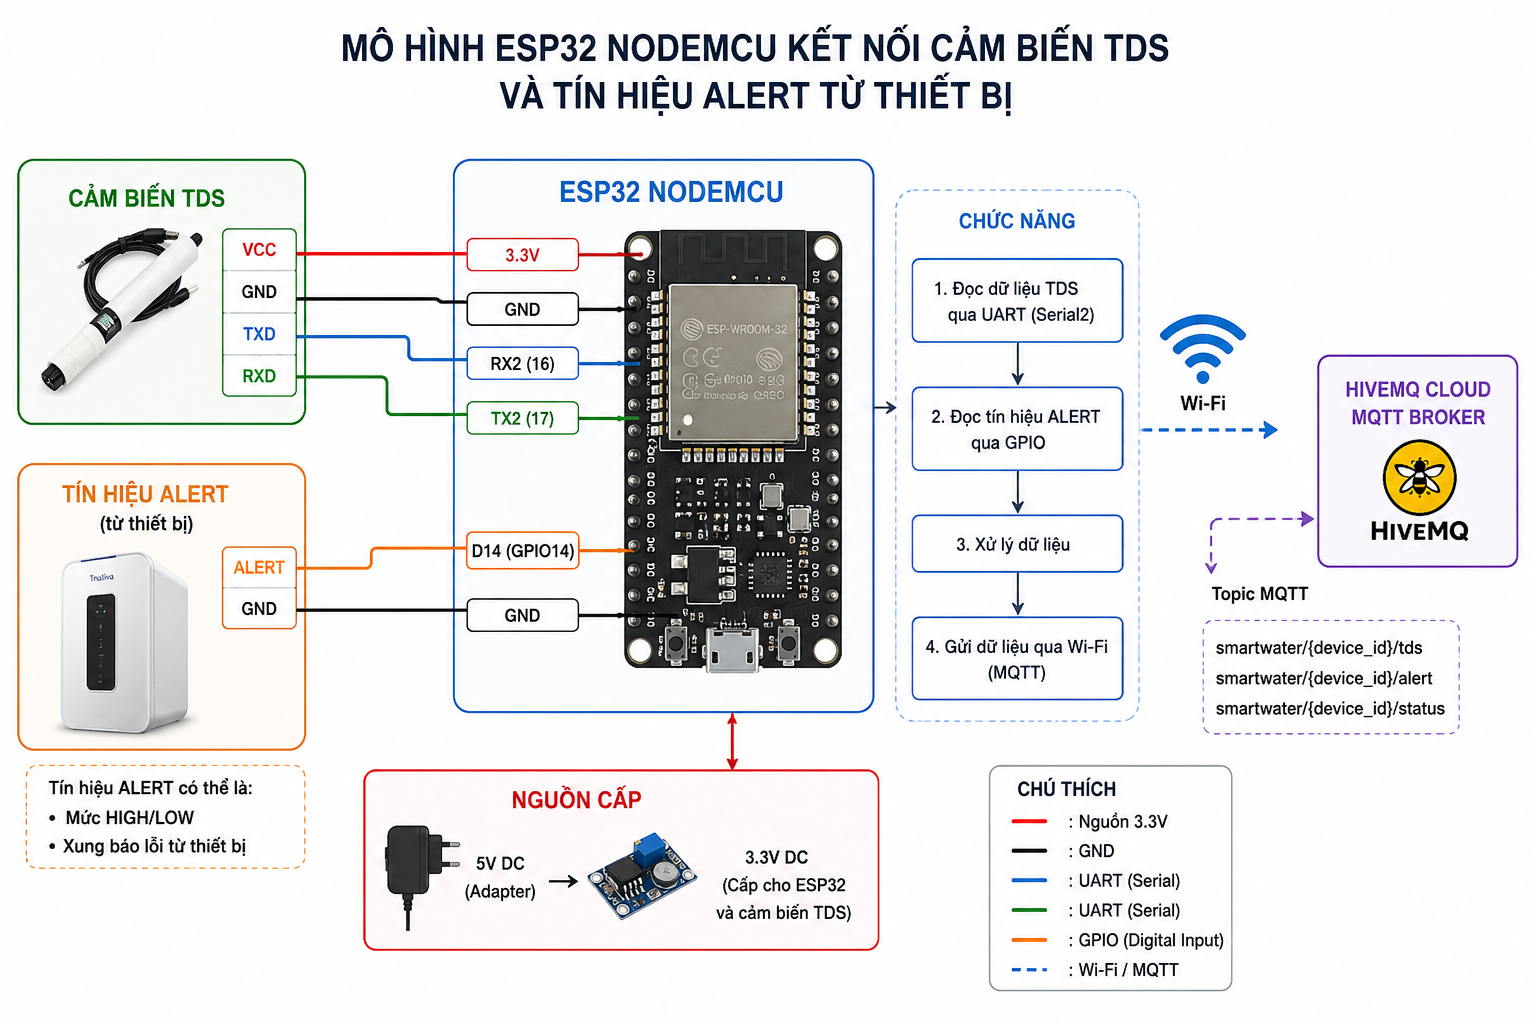
\includegraphics[width=0.9\textwidth]{include/image/ESP32-NodeMCU.png}
    \caption{Mô hình ESP32 NodeMCU thu thập dữ liệu từ cảm biến TDS và tín hiệu Alert của máy lọc nước Truliva}
    \label{fig:esp32-node}
\end{figure}

\subsubsection*{4.3 Kết quả đạt được}

Sau khi hoàn thành các công việc trong tuần 4, sinh viên đã đạt được các kết quả sau:

\begin{itemize}
    \item Khảo sát và nắm được cấu trúc phần cứng của máy lọc nước Truliva, xác định chức năng của các thành phần chính như bo điều khiển, bo hiển thị, cảm biến và các cơ cấu chấp hành.

    \item Phân tích được kiến trúc điều khiển của thiết bị, xác định mối liên kết giữa bo điều khiển UR S61298 và bo hiển thị UR S61296, đồng thời nhận diện các giao tiếp và tín hiệu phục vụ quá trình truyền dữ liệu.

    \item Đánh giá các phương án thu thập dữ liệu từ thiết bị, phân tích ưu điểm và hạn chế của từng giải pháp, từ đó xác định phương án sử dụng ESP32 làm bộ thu thập dữ liệu độc lập là phù hợp với yêu cầu của dự án.

    \item Hoàn thành thiết kế sơ bộ mô hình kết nối giữa ESP32 NodeMCU, cảm biến TDS và tín hiệu Alert của thiết bị, tạo nền tảng cho việc triển khai phần cứng ở các giai đoạn tiếp theo.

    \item Nghiên cứu phương thức truyền dữ liệu sử dụng giao thức MQTT và xây dựng kiến trúc kết nối giữa ESP32, HiveMQ Cloud và hệ thống Device Monitor phục vụ quá trình thu thập và lưu trữ dữ liệu telemetry.

    \item Chuẩn bị đầy đủ cơ sở kỹ thuật cho giai đoạn lập trình ESP32, thu thập dữ liệu thực tế và tích hợp với hệ thống SmartWater trong các tuần tiếp theo.
\end{itemize}